\section{Úvod do problematiky}
Saliency a teda detekcia významných oblastí je využívaná v rôznych oblastiach.Počínajúc automatizáciou, modely významných oblastí (anglicky saliency modelov) sú tažiskom pri segmentácií obrazu alebo detekcií špecifických objektov.
Od saliency modelov sú taktiež závislé aj programi ovládajúce zabezpečovacie zariadenia.
Tu saliecny modely zužujú možnosti a proaktívne upozorňujú na podozrivé situácie.
Až po reklamu, kde je vyzuálna pozornosť klúčovým parametrom, čo môže rozhodnúť o úspechu produktu, veď aký význam by mala reklama, kde si nevšimnete prezentovaný produkt alebo si všimnete iba jeho "menej" dokonalé časti.
\section{Metody pre statické obrázky}
Algoritmy pre statické obrazy tvoria základ všetkých saliency modelov a tvoria najstaršiu oblasť výskumu.
V tejto časti uvediem prehľad algoritmov pre výpočet saliency modelov od najjednoduchších cez najznámejšie až po nejefektívnejšie.
Na záver uvediem porovnanie všetkých metód pomocou všeobecne uznávaných metrík a dát získaných zo zariadení merajúcich pohyb očí používateľa (eyetrackera).
\subsection{Baseline Center}\label{section:caseline-center}
Baseline center je triviálny model,  ktorý sa vypočítava pomocou Gaussovej krivky vzľadom na pomer strán čím, predpokladá salientné oblasti presne v strede obrazu.
Nezachytáva však žiadne sémantické aspekty videa ako ani podvedomé informácie vnímanania obrazu iba rozlíšenie dané optikou skenujúcou scénu.
\subsection{Hrany}
Skupina algoritmov využívajúca význačné prechody v obraze inak nazývane hrany.
Metódy tohoto typu sú vyžívané hlavne v prírodných scénach, kde nie je (hlavne sémanticky) význačný objekt.
Takéto metódy sa zakladajú priamo na štúdiu fyziologických vlastností ľudského vyzuálneho systému.
Následná imitácia procesov odohrávajúcih sa na sietnici viedla ku vzniku saliency modelov, generujúcich plausibilné výsledky\cite{edges-1}.
\subsection{Ittiho model}
Najznámejším modelom pre výpočet významných oblastí pre statické farebné obrazy je ittiho model navrhnutý v roku 1998.
Model zakladá na rozložení obrazu na 3 základné charakteristiky obrazu a to farbu, intenzitu, orientáciu.

\begin{figure}[H]
 \centering
 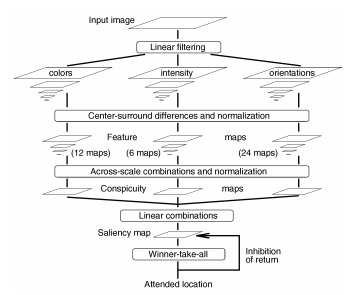
\includegraphics[width=7cm]{pics/itti-1.png}
 \caption{Itti model general workflow.}\label{wrap-fig:1}
\end{figure}
\vspace{10mm}

Chrakteristika farby obsahuje 12 máp (šedotónové obrazy), pričom model používa farebný model RGB.
Nazačiatku sa vypočíta intenzita podľa vzťahu \begin{math} I = (R+G+B)/3\end{math}.
Pomocou mapy I sa následne normalizujú všetky farebné kanály modelu RGB.
Model extrahuje 4 farebné kanály červený (r), zelený (g), modrý (b), zltý (y) a pomocou Gausvých pyramíd vytvorí 3 rôzne mapy každej farebnej zložky separátne.
Červená zložka sa počíta difenčným spôsobom ako \begin{math} R = r - (g + b)/2 \end{math}, zelená ako \begin{math} G = g - (r + b)/2 \end{math}, modrá ako \begin{math}B = b - (r + g)/2\end{math} a žltá ako \begin{math}Y = (r + g)/2 - |r - g|/2 - b\end{math}.
Chrakteristika intenzity obsahuje 6 máp.
Získaná je pomocou orientovaných gáborových filtrov s orientáciou 0\degree, 45\degree, 90\degree, 135\degree.
Dokopy 42 máp charakteristík je následne linárne skombinovaných do jednej saliency mapy\cite{itty-98}.


\subsection{Spektralne rezidua}
Medtóda využíva princím, že potláča štatisticky často opakujúce sa časti obrazu a do popredia stavia časti obrazu ktoré sa štatisticky odlišujú od ostatných.
Na detekciu používa rýchlu fourierovu transformáciu.
Pomocou nej rozdelí obrázok na amplitúdovú čast a fázovú čast.

\begin{figure}[H]
  \centering
  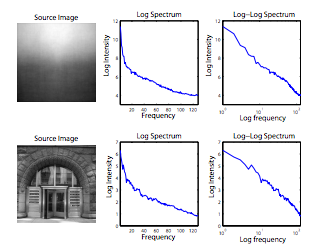
\includegraphics[width=10cm]{pics/spectral-rezidual-1.png}
  \caption{Príklad rozloženia typovo rôznych obrázkov}\label{wrap-fig:2}
\end{figure}
\vspace{10mm}

Amplitúdová zložka sa následne vyhladí, čím sa do popredia dostanú iba informácie, ktoré sa vymykajú z priemeru.
Odčítaním od pôvodnej amplitúdoje zložky dostaneme iba časti obrazu, ktoré sú významné \cite{spectral-rezidual}.
\subsection{Sun Model}
Sun model (Saliency Using Natural statistics) sa snaží symulovať potencionálne ciele sledovania ludského vyzuálneho systému.
Model aktívne ohodnocuje tieto ciele odhadom pravdepodobnosti vzhľadom na všetky pozorované charakteristiky.
Charakteristiky sú spracovávané separátne a teda model nepočíta s chrakteristikami navzájom sa ovplynujúcimi.
Údaje získané zo všetkćyh charakteristík  následne spracuje šatisticky.
Model zakladá hlavne na Bayesovom pravidle[TODO referencia?].
Za výsledok hľadania potom udáva asimetrie v týchto štatistických štruktúrach\cite{sun-1}.
\subsection{Rare Model}
Výrazná vätšina modelov pozornosti typy bottom-up funguje ustáleným postupom, kde sa z pôvodného obrazu extrahuje definovaná množina chrakteristík paralelne a tie následne kombinujú alebo inak použiju na výpočet výslednej mapy pozonosti.
Rare model narvhuje sekvenčnú architektúru, kde z pôvodného obrázku extrahuje nízko úrovňové príznaky.
Následne na výsledkoch sériovo vykonáva extrakciu dalších príznakov (v literatúre nazívané mid-level).
Nakoniec ako posledný krok spojí a normalizuje výsledné chrakteristiky do konečnej mapy významných oblastí.
Rare model ako nízko úrovnové chrakteristiky používa jas a colorimetrické rozdieli (ako farebný model používa YCbCr) a následne na mapách rozložených žložiek farebného modelu detekuje orientáciu pomocou gáborových filtrov\cite{rare-1}.
Po extrakcii všetkých charakteristík použije iteratívnu metódu pre optimálne kvantovanie založenú na metóde Otsu\cite{otsu}.
Na takto upravenom vstupe sa následne vyhľadávajú vzácne (z angl. rare) oblasti obrazu.
Metóda preskúmala možnosti nesekvenčnej extrakcie príznakov z obrazu bol novým prístupom v oblasti modelov pozornosti.

\begin{figure}[H]
  \centering
  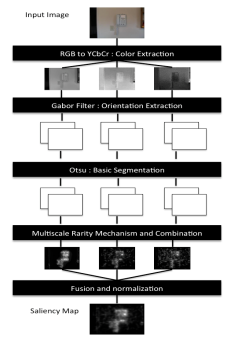
\includegraphics[width=6cm]{pics/rare-1.png}
  \caption{Rare model workflow}\label{wrap-fig:3}
\end{figure}

\section{Metody pre videá}
Video obsahuje rozsiahlejšie možnosti ako iba obrazová informácia, pribúdajú ďalšie rozmery ako je pohyb objektov na obraze alebo vplyv zvuku na ľudské vnímanie.
Avšak oproti obrazu obsahuje je potrebné spracovávať vedšie množtvo
dát.
Navyše vo vetšine algoritmov využívajúcich saliency modely je potrebné aby model dával výsledky v reálnom čase.
Používané hlavne v oblasti zabezpečovacej techniky.
\subsection{Zohladnenie audio informácie}
Saliency modely využívaju rôznorodé druhy príznakov a to od geneticky zakorenených ako sú prechody farieb, alebo intenzít, až po sémantické príznaky ako je detekcia tváre \cite{salient-faces}.
Majoritná vedšina saliency modelov využíva iba obrazovú zložku ale zvuková stopa býva ponechaná stranou ale úplne zanedbaná.
Použitie zvuku je známimtrikom filmovej scény uz desatročia, kde režiséri posilňujú kontrolu nad diváckou pozornosťou práve pomocou zvukového doprovodu.
Prvé štúdie sa zaoberali detekciou reči a tváre, kde je spojitosť jednoznačná \cite{sound-1}.
Neskoršie štúdie dokazujú korelácie aj na všeobecnejšej úrovni a pokusy o extrakciu samotnej charakteristiky zo zvukovej stopy\cite{sound-coutrot-1}.
Tieto pokusy viedli aj k zostaveniu modelov zohladňujúc zvukovú stopu ako samostatnú charakteristiku spolu s kombináciou s nízko-urovnovými príznakmi obrazu \cite{sound-courot-2}.

\begin{figure}[H]
  \centering
  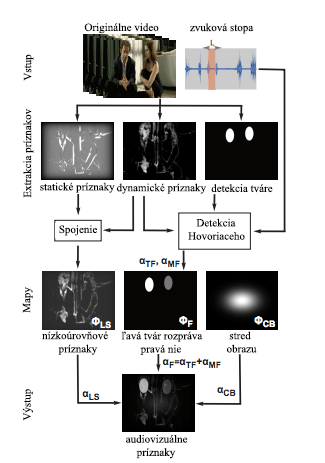
\includegraphics[width=10cm]{pics/courot-1.png}
  \caption{Audiovisual model workflow.\cite{sound-courot-2}}\label{wrap-fig:4}
\end{figure}
\vspace{10mm}

Model extrahuje video na sekvenciu obrazov (framy) a audio stopu v tvare grafu vlnovej dĺžky.
Potom extrahuje 3 typy rôznych chrakteristík.
Nízko-úrovňové príznaky založené na biologicky inširovaných saliency modeloch rozdelených na dynamickú časť a satickú časť.
Statická časť sa zameriava na najasnejšie a najkontrastnejšie časti obrazu.
Dynamická časť sa zameriava na relatívny pohyb objektov vhľadom na pozadie (eliminácia pohybu kamery).
Tieto 2 časti sa nakoniec spoja
Dalšou chrakteritikou použitou v tomto modeli je detekcia tváre.
Každý objekt klasifikovaný ako tvár je v saliency mape nahradený oválnym objektom, intenzita daných objektov je daná pomocou metódy Speaker Diarization, ktorá detekuje podľa zvukovej stopy objekt ktorý generuje zvuk.
Metóda predpokladá striedavú konverzáciu n objektov oddelenú pauzou.
Následne spojí vyššie spomínané charakteristiky do jednej výslednej mapy.
Ako posledný krok preloží cez celú mapu baseline center model popísaný v časti \ref{section:caseline-center}.

\subsection{Detekcia pohybu}
V tejto časti sa zmeriame na segmentáciu objektov ktoré sa na scéne pohybujú.
Metódy tohoto typu sa snažia vyzualizovať 3D prostredia (v našom prípade disponujeme výskou, širkou, časom) na 2D výstup (obrazový výstup).
Takáto informácia dokáže priblížíť výpočtové modely bližšie k realite.
Ľudský vyzuálny systém totiž nepoužíva iba 2d vstup (ako to prebieha vo drvivej vetšine metód na výpočet významných oblastí).
Taktéto obrazy sú v ľudskom vyzuálnom systéme vysoko hodnotené.
Dôvody, prečo takto ľudský vyzuálny systém pridáva prijoritu práve takýmto oblastiam možeme nájsť v antropológií (citacia?).
Vysvetlenie je jednoduché a to snaha zabezpečit bezpečné prostredie okolo seba a všetko pohybujúce sa narušuje pocit bezpečnosti.
V nasledujúcom texte rozoberieme 2 najpožívanejšie algoritmy používané na detekciu oblastí pohybu v obraze a výpočet vektoru posunu.
Výpočet vektoru pohybu je však iba projekcia 3D vstupných dát do 2D obrazu, nemusí vždy reprezentovať iba pohyb.
Prvým z nich bude LUCAS KANADE\cite{lucas-kanade}, a druhým Horn Schunck\cite{horn-schunck}.
Oba tieto algoritmi používajú jeden spoločný predpoklad a to, že jas daného objektu sa časom nemení.
To značí, že objekt sa na scéne može presunúť  ale svoj jas nemôže zmeniť.
Matematicky vyjadrené I(x(t),y(t),t) je obrazová dvojrozmerná funkcia, ktorá sa mení vzhľadom na čas.
Kedže sa jas obrazu nemení môžeme povedať, že platí:
\begin{equation}
  I(x + dx/dt \sigmat ,y + dy/dt \sigmat, t + \sigmat) = I(x,y,t)
\end{equation}
Z čoho je ľahko odvoditeľné, že:
\begin{equation}
  dI/dt = \sigmai/\sigmax dx/dt + \sigmai/\sigmay dy/dt + dI/dt  =  0
\end{equation}

\subsection{Lucas Kanande}
Algoritmus prvotne vznikol ako návrh pre časovú optimalizáciu problému výpočtu vektoru posunu medzi dvomi krivkami.
Povodné intitívne riešenie vyžadovalo \begin{math} O(M^2 * N^2) \end{math} času pre výpočet daného vektoru ak M,N bolo rozlíšenie daného obrazového vzoru.
Vtedy nahvrhovaná optimalizácia vyžadovala zadanie rozsahu hladania, pomocou ktorého sa vypočítali diferencie pre celý obraz a pre ďalšiu iteráciu sa rozsah vypočítal pomocou horolezeckého algoritmu.
Metóda Lucas Kanade využíva priestorový gradient pre výpočet nových hodnôt a zároveň upravuje hodnotu rozsahu pri výpočte kažkého obrazového pixelu v obraze a nie iba po výpočte celého obrazu.
Pomocou takejto úpravu naivného algortimu sa časová zložitosť zlepšila na \begin{math} O(M^2 log N) \end{math}\cite{lucas-kanade}.

\begin{figure}[H]
  \centering
  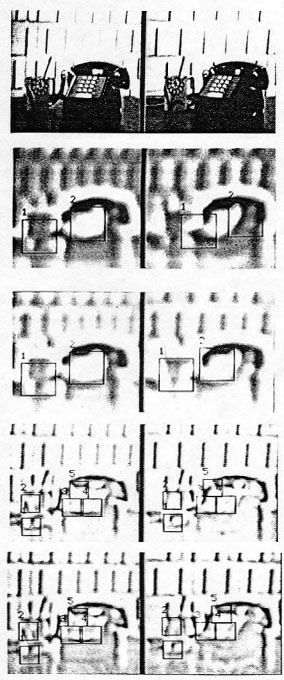
\includegraphics[width=10cm]{pics/lukas-kanade.jpg}
  \caption{Vyzualizacie výsledkov algoritmu Lucas-Kanade vždy po 1 iterácíí}
\end{figure}
\vspace{10mm}

\subsection{Horn-Schunck}
Metóda Horn-Schunck bola prvá, kde bola použitá metóda variácie na výpočet optického toku.
Táto globálna metóda priniesla výpočet  konštanty pre obmedzenie plynulosti optického toku.
Algoritmus používa 2 základné parametre: Počet iterácií a vyhladzovaciu konštantu.
Počet iterácií určuje dĺžku (počet cyklov) simulácie, vyhladzovacia konštanta je použitá po každom cykle simulácie kvôli zjemneniu prechodov a výpočet optimálneho optického toku.

\begin{figure}[H]
  \centering
  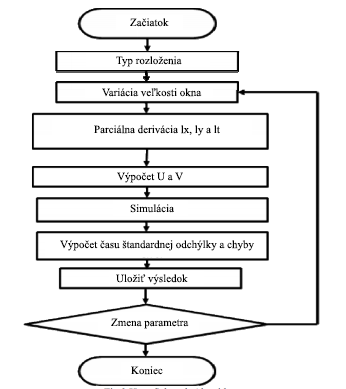
\includegraphics[width=7cm]{pics/horn-schunck.png}
  \caption{Vyzualizácia pracovného postupu metódy Horn-Schunck}
\end{figure}
\vspace{10mm}

\section{Metriky úspešnosti}
Metriky úspešnosti sú algoritmy pre čo najpresnejšie vyjadrenie presnosti modelov v meratelných jednotkách.
Takýto algoritmus dostáva na vstupe čisté dáta z eye trackera.
Tieto je potrebné predspracovať z dôvodu, že každý výrobca poskytuje iné zariadenia na hardwarovej úrovni a výrobcovia neštandardizujú výstup do jednotnej formy.
Následne je potrebné vytvoriť mapy fixácií ktorá sa používa ako jeden zo vstupných parametrov v algoritmoch rátajúcich metriky úspešnosti.
\\
Metriky úspešnosti možno rozdeliť do 3 štandardných skupín podľa druhu hodnôt na ktorý porovnávajú reálne dáta (v literatúre nazívané ground truth) s vygenerovanýmy mapamy význačných oblastí\cite{metrics-1}.
\begin{enumerate}
  \item\textbf{Založené na porovnávaní hodnôt} - NSS, Percentile, Pf
  \item\textbf{Založené na vyhodnocovaní vzdialenistí} - AUC-Judd, AUC-Zhao, AUC Borji, AUC-Li
  \item\textbf{Založeneé na distribúcií} - KL-Div, EMD, CC, SRCC
\end{enumerate}

\subsection{NSS}
NSS (Normalized Scanpath Saliency) metrika narvrhnutá v roku 2005 ktorej autormi sú R.
J.
Peters a L.
Itti.
Metrika zakladá na ohodnotení salientných oblastí vzľadom na pozíciu fixácií samostatne a následná normalizácia podľa počtu fixácií.
\\
Pre každú fixáciu používa vzťah
  \begin{equation}
    NSS(p) =  (SM(p)-\SI{}{\micro}_{SM}) / 	\sigma_{SM}
  \end{equation}
Kde SM je mapa význačných oblastí a p je bod danej fixácie pre ktorú sa hodnota vypočítava.

Pričom mapa fixácií SM je normalizovaná tak aby nadobúdala nulovú strednú hodnotu a zároveň jednotkovú štandardnú dochýlku.
Metrika NSS nadhodnocuje ak je saliency mape minimálna rozmanitosť hodnôt (malý rozdiel medzi hodnotami fixácií a strednou hodnotou), pretože v takomto prípade nebude model dostatocne odhonotený, ak nájde presné pozície v prípade, že odchýlka je malá, alebo
rozdiel medzi hodnotami fixácie a strednou hodnotou je vysoké.
Finálna hodnota NSS metriky je určená priemerom hodnôt pre všetky fixácie\cite{metrics-1}.

\begin{equation}
  NSS = 1/N * \sum_{p=1}^{N}NSS(p)
\end{equation}

\subsection{AUC-Judd}
Metrika je clasická AUC ktorú navrhol Judd \cite{auc-judd}.
Ako prvé sa pixely označené ako fixácie spočítajú s rovnakým počtom náhodných pixelov vybraných z mapy význačných oblastí a pixely sú nakoniec považované za klasifikátor úspešnosti.
Následuje prahovanie zvolenou hodnotou, pixely ktoré sú menšie ako prahovacia hodnota sú pokladané za pozadie obrazu a pixely ktoré majú hodnotu vyššiu sú pokladané ako fixácie.
Pre ľubovolne zvolenú prahovaciu hodnotu sú niektoré výsledné oblasti manuálne označené ako pozitívne (True Positives), pobobne niektoré oblasti ktoré nie sú označené ako fixácie sú manuálne označené ako falošne pozitívne (False Positive).
Tieto operácie sú zopakované tisíc krát, nakoniec sa vyzualizuje pomocou ROC krivky a plocha pod pod krivkou (Area Under the Curve preto AUC) je výsledným klasifikátorom, ktorého ideálna hodnota je 1.
Hodnota náhodného výberu je 0.5.

\subsection{KL-Div}

Každý projekt vytvárajúci model významných oblastí si volí vlastné metriky úspešnosti, podľa ktorých sa určuje úspešnosť daného modelu.
Pre meranie úspešnosti modelov je okrem samotných algoritmov pre meranie úspešnosti potrebné zabezpečiť dostatočne rôznorodú skupinu testovacích dát tkz.
datasetov.

\section{Refenčné datasety}
Dataset je testovacia množina, ktorá sa snaží obsiahnuť dostatočne rôznorodé vzorky vhodné pre komplexné testovanie.
Pri zostavovaní datasetov sú dôležité nielen videá ale eyetracker data alebo nejakým spôsobom zverejnené fixácie, aby bolo možné výsledky validovať pomocou vyššie uvedených metrík.
Poslednou charakteristikou datasetu je množsto ľudí na ktorých boli dané viedeá nahrávané.
\\ Príklady datasetov:
\begin{itemize}
	\item \textbf{RSD}\cite{rsd}
	\item \textbf{SAVAM}\cite{savam}
	\item \textbf{AUDITORY DATASET}\cite{courot-dataset}
\end{itemize}

\subsection{RSD}
Regional Saliency Dataset je zaujímavý o čo najobšírnejšie testovanie je rozdelený do 4 hlavných kategórií: \\
\begin{itemize}
	\item \textbf{bezpečnostné záznamy} - Štadardné záznamy z bezpečnostných kamier obsahujú statické pozadie a salientné pohybujúce sa objekty.
Pre túto čast datasetu vyžili záznamy z projektu CAVIAR\cite{rsd-caviar}.
	\item \textbf{Grafika} - Použité animované filmy/seriáli ktoré obsahujú 2D aj 3D grafiku.
  \item \textbf{Prirodzené videá s prvkami grafiky} - Prirodzené videá  podobné bezpečnostným ale s prvkami umelo vložených priamo do obrazového kanálu.
  \item \textbf{Prirodzené videá} - Videá bez pridaných grafických prvkov, tak ako boli nasnímané kamerou.
\end{itemize}

Na vyznačenie zaujímavých oblastí nezvolili techniku (eyetracke) ale manuálne vyznačovanie zaujímavých oblastí pomocou používateľov.
Výskumu sa zúčastnilo 17 mužov 6 žien medzi 10-23 rokov, na označení každého z videa sa podielalo 10-23 ludí.

\begin{figure}[H]
 \centering
 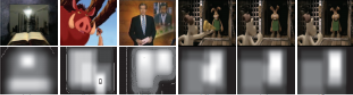
\includegraphics[width=7cm]{pics/rsd.png}
 \caption{Ukážka z každej kategórie videa s oznčenými významnými oblastami}
\end{figure}
\vspace{10mm}

\subsection{SAVAM}
SAVAM (Semiautomatic Visual-Attention Modeling) je dataset nahrávaný priamo pomocou eyetrackera pri sledovaní videí v HD rozlíšení pričom každému nahrávanému používateľovy sú pridelené dáta separátne pre kažké oko.
Dokopy obsahuje 13minút videa, ktoré bolo otestované na 50 používateľoch rôzneho veku.
Dataset je rozdelený na videá z filmov, ukážky z komerčných videí a stereoskopické videá.
SAVAM taktiež poskytuje všetky raw dáta z eyetrackere ako aj vizualizácie daných dát\cite{savam}.

\subsection{AUDITORY DATASET}
Posledný dataset ako jediný poskytuje aj audio informácie ktoré je možné ďalej spracovávať.


\section{Porovnanie štandardných Metód}
Porovnávanie metód je štandardne publikované formou ucelených benchmarkov.
Príkladom takéhoto banchmarku je mit saliency benchmark\cite{mit-saliency-benchmark}, ktorý sa snaží zgrupovať a porovnávať obrazové modeli pozornosti.
V tejto sekcií ďalej uvedieme iba vyualizácie všetkých vyššie uvedených metód, pomocou obrázkov z testovaného videa (vybrané z vyššie uvedených datasetov) a im prislúchajúcich saliency máp vygenerovaných pomocou popísaných modelov alebo metód.
Ďalej ich porovnanie pomocou výpočtových parametrov v tabulke.

\begin{figure}[H]
 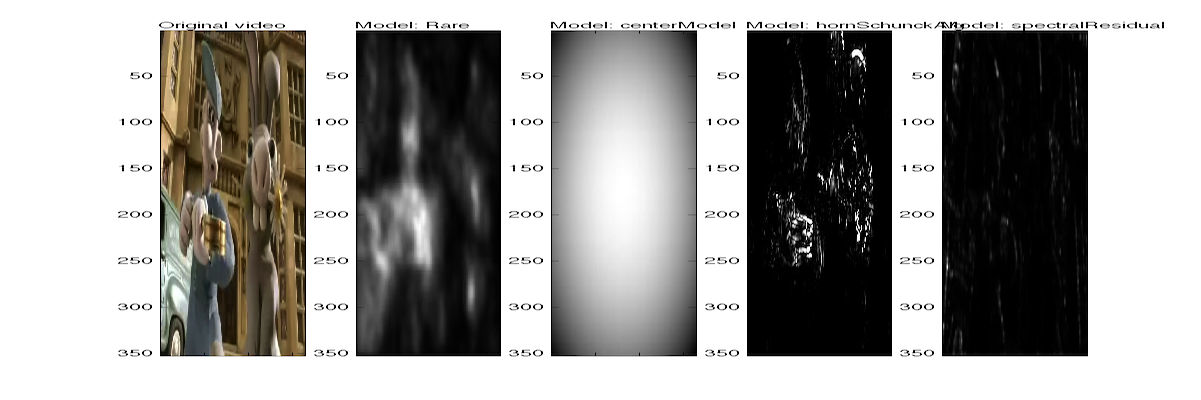
\includegraphics[width=17cm]{pics/porovnanie-1.png}
 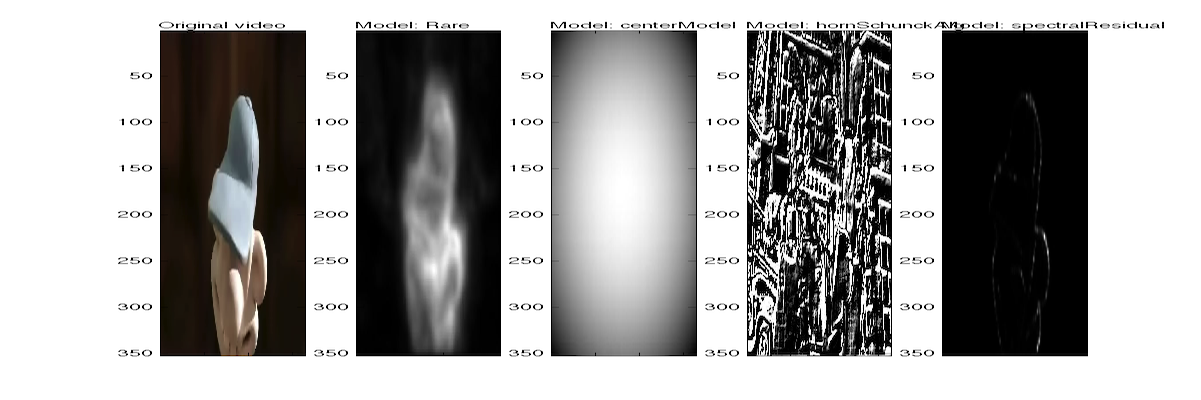
\includegraphics[width=17cm]{pics/porovnanie-2.png}
 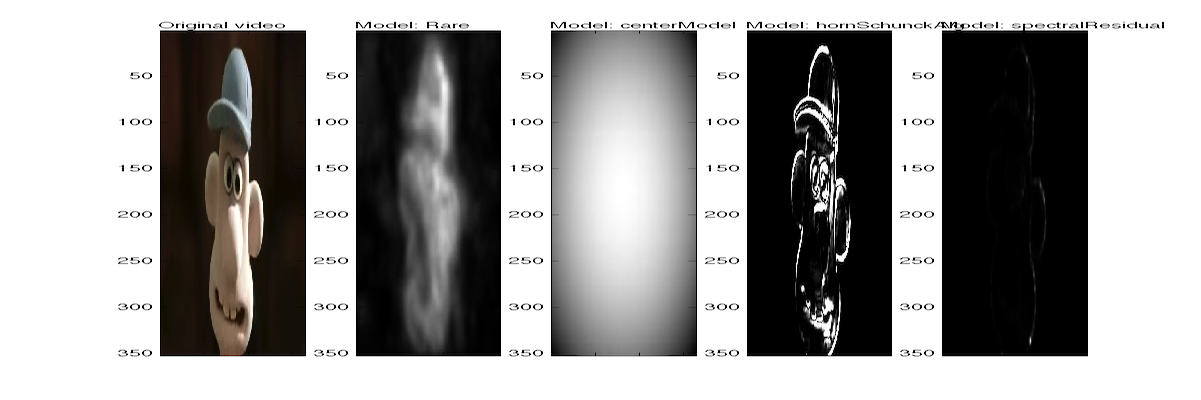
\includegraphics[width=17cm]{pics/porovnanie-3.png}
 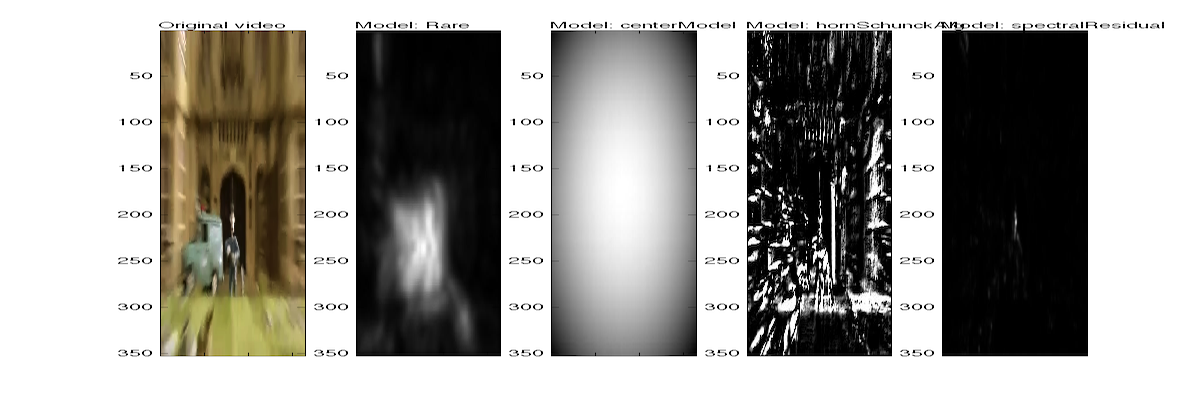
\includegraphics[width=17cm]{pics/porovnanie-4.png}
 \caption{Porovnanie vybraných algorithov na videu z datasetu RSD.}
\end{figure}
